\documentclass[main.tex]{subfiles}
\begin{document}
\chapter{Ananlyse de mélanges bi-gaussien}
\lettrine[lines=2, lhang=0.33, loversize=0.25]{D}{ans} tout ce chapitre dédié à l'analyse d'un mélange bi-gaussien sous toutes les coutures, nous considèrerons les mêmes notations que celles utilisées dans le chapitre REFF ??? \todo[noline]{ref chap}. Une gaussienne normalisée est décrite par son écart-type~$\sigma$ et son centre~$c$ (qui est aussi l'espérence notée plutôt $\mu$ lorsqu'on fait des statistiques). Ici on en considère deux~:

\section{Propriétés d'une gaussienne}
On considère une gaussienne définie selon deux paramètres, son écart-type~$\sigma$ et son centre~$c$ (qui est aussi l'espérence notée plutôt $\mu$ lorsqu'on fait des statistiques)~:
\begin{equation}
\label{eq:anxe_gaussienne}
g(x)=\dfrac{1}{\sigma \sqrt{2\pi}} \exp\left( \frac{-1}{2}  \left(  \dfrac{x-c}{\sigma} \right)^2  \right).
\end{equation}

\begin{prop}
Les dérivées d'une gaussiennes sont données par~:
\begin{itemize}
\item pour la dérivée première~: $g'(x)= -\dfrac{x-c}{\sigma^2}g(c), $
\item pour la dérivée seconde~: $g''(x)= \dfrac{(x-c+\sigma)(x-c-\sigma)}{\sigma^2}g(c). $
\end{itemize}
\end{prop}

Une gaussienne étant toujours positive (car l'exponentielle l'est toujours), la propriété ci-dessus permet de mettre en avant le rôle des points d'abscisse~$c-\sigma$ et~$c+\sigma$, lieu des changements de concavité (annulation de la dérivée seconde).

\begin{prop}
\label{prop:integ1}
La gaussienne $g$ définie ci-dessus est normalisée \ie
\begin{equation}
\label{eq:anxe_integ_gauss}
\int\limits_{-\infty}^{+\infty} g(x) \dx = 1
\end{equation}
\todo[noline]{demo integ = 1}
\end{prop}


\section{Comment s'intersectent deux gaussiennes ?}
Dans cette section on ne considère plus $g$ comme une seule et unique gaussienne, mais comme un mélange bi-gaussien. Il est décrit par la somme de deux gaussiennes pondérées par les poids~$w_1$ et $w_2$~:
\begin{equation}
\label{eq:anxe_bi_gauss}
g(x)= w_1 g_1(x)+ w_2 g_2(x) \quad \textrm{avec} \quad w_1 + w_2=1,
\end{equation}
où $g_1$ et $g_2$ sont des gaussiennes définies respectivement en fonction des paramètres~$c1,\sigma_1$ et~$c_2,\sigma_2$ via la formulation~\eqref{eq:anxe_gaussienne}. Comme la somme des poids est de 1, la Propriété~\ref{prop:integ1} reste valable pour un mélange gaussien.

Comme présenter dans le chapitre REFF ??, le calcul de l'intersection des deux composantes se résume à~:
\begin{equation}
\begin{aligned}
\label{eq:anxe_polynome}
g_1(x)=g_2(x) \quad \Longleftrightarrow & \quad  Ax^2 + 2B'x + C =0 \\
{\rm avec :} \quad &A=\sigma_2^2 - \sigma_1^2, \\
& B'=c_2\sigma_1^2-c_1\sigma_2^2,\\
& C= c_1^2\sigma_2^2-c_2^2\sigma_1^2 +  2\sigma_1^2\sigma_2^2 \ln( h_2 / h_1 ).
\end{aligned}
\end{equation}
Le discriminant réduit de ce polynôme est donné par~:
\begin{equation}
\label{eq:anxe_discr_reduit}
\Delta' := B'^2 - AC = \sigma_1^2 \sigma_2^2 \left[ (\Delta c)^2 - 2(\sigma_2^2-\sigma_1^2) \ln (h_2/h_1)  \right].
\end{equation}
On peut réécrire cela en posant $\bar{c}=(c_1+c_2)/2$, $\Delta c = c_2-c_1$ et $\sigma_2=\sigma$ avec $\sigma_1=\beta \sigma$. Ceci donne~:
\begin{equation}
\begin{aligned}
\label{eq:anxe_polynome2}
&g_1(x)=g_2(x) \quad \Longleftrightarrow  \quad  Ax^2 + 2B'x + C =0 \\
{\rm avec :} \quad &A=1-\beta^2, \\
& B'=\bar{c}(\beta^2-1)+ \frac{\Delta c}{2}(1+\beta^2),\\
& C= (\bar{c}^2+(\Delta c)^2 ) (1-\beta^2) -\bar{c}\Delta c (1+\beta^2) + 2 \beta^2 \sigma^2 \ln \left( \frac{1-w}{w}\beta \right).
\end{aligned}
\end{equation}
Si $\sigma_1 \neq \sigma_2$ \ie $\beta \neq 1$, alors on peut simplifier  l'écriture :
\begin{equation}
\begin{aligned}
\label{eq:anxe_polynome3}
&g_1(x)=g_2(x) \quad \Longleftrightarrow  \quad  x^2 + 2B'x + C =0 \\
{\rm avec :} & B'=\frac{\Delta c}{2} \frac{1+\beta^2}{1-\beta^2}-\bar{c},\\
& C= \bar{c}^2+(\Delta c)^2 -\bar{c}\Delta c \frac{1+\beta^2}{1-\beta^2} + 2 \frac{\beta^2}{1-\beta^2} \sigma^2 \ln \left( \frac{1-w}{w}\beta \right).
\end{aligned}
\end{equation}
Le discriminant réduit de ce polynôme est donné par~:
\begin{equation}
\label{eq:anxe_discr_reduit}
\Delta' := B'^2 - AC = \sigma_1^2 \sigma_2^2 \left[ (\Delta c)^2 - 2(\sigma_2^2-\sigma_1^2) \ln (h_2/h_1)  \right].
\end{equation}



\begin{thm}\label{thm:anxe_pt_unique}
Il ne peut y avoir qu'un seul et unique point d'intersection situé entre les centres des deux composantes d'un mélange bi-gaussien.
\end{thm}

\begin{proof}
Considérons la différence des deux composantes $d(x)=g_2(x)-g_1(x)$ et supposons sans perte de généralité que $c_1<c_2$. On a alors~:
$$d'(x) = \frac{c_2-x}{\sigma_2^2}g_2(x) - \frac{c_1-x}{\sigma_1^2} g_1(x) >0 \quad \forall x \in [c_1; c_2] $$
Ainsi $d$ est strictement croissante sur $[c_;,c_2]$. La fonction $d$ étant de plus continue, elle ne peut donc s'annuler qu'au plus une fois sur l'intervalle $[c_1;c_2]$.
\end{proof}

Une autre démonstration que nous allons présenter, consiste à considérer la valeur des points d'intersections eux mêmes (on se place dans le cas où ces points existent), donnée via le polynôme~\ref{eq:anxe_polynome}~:
\begin{equation}
\label{eq:anxe_racines}
x_\pm = -B' \pm \sqrt{\Delta'},
\end{equation}
et à montrer par l'absurde que les deux racines ne peuvent être toutes les deux comprises entre $c_1$ et $c_2$. Tout d'abord commençons par énoncé deux lemmes.
\begin{lemme} \label{lem:distance_milieu}
Un point $x$ appartient à un intervalle $[c_1;c_2]$ \ssi sa distance avec le milieu de l'intervalle est inférieure à la moitié de la longueur de cet intrevalle~:
\begin{equation}
x \in [c_1;c_2]
 \quad \Longleftrightarrow \quad 
 | x - \bar{c}  | \leq \frac{\Delta c}{2}  \quad \textrm{avec} \quad \bar{c}=\frac{c_1+c_2}{2} \ \textrm{et} \ \Delta c = c_2-c_1.
\end{equation}
Le même résultat est fourni pour un intervalle ouvert, avec des inégalités strictes.
\end{lemme}
\begin{proof}
\begin{align*}
 | x - \bar{c}  | \leq \frac{\Delta c}{2} & \Longleftrightarrow \frac{-\Delta c}{2} \leq x-\bar{c}\leq \frac{\Delta c }{2}  \Longleftrightarrow \frac{-\Delta c}{2} +\bar{c}\leq x\leq \frac{\Delta c }{2} +\bar{c} \\
 &\Longleftrightarrow c_1 \leq x \leq c_2 \Longleftrightarrow x \in [c_1,c_2]
\end{align*}
De plus, on peut appliquer exactement le même raisonnement avec des inégalités strictes.
\end{proof}
\begin{lemme} \label{lem:qtes_negatives}
Deux quantités $a$ et $b$ sont toutes deux négatives \ssi leur produit est positif et leur moyenne est négative~:
$$ ( a<0\ \textrm{et}\ b<0 ) \quad \Longleftrightarrow \quad \left( ab>0\ \textrm{et}\ \frac{a+b}{2}<0  \right).$$
\end{lemme}
\begin{proof}
L'implication $\Rightarrow$ est immédiate. La réciproque est donnée par le fait que $ab>0$ implique que $a$ et $b$ soit de même signe. S'ils sont tous les deux positifs, alors cela implique que leur moyenne est positif. Ce qui est contradictoire, donc $a$ et $b$ sont tous les deux négatifs.
\end{proof}
\begin{lemme}
\label{lem:ineg} Quelquesoit un réel $\beta$ différent de -1 ou 1 a l'égalité suivante 
\begin{equation}
\forall \beta \in \reel \setminus \{ -1; 1 \}, \qquad  \left| \frac{1+\beta^2}{1-\beta^2} \right| \geq 1
\end{equation}
avec égalité seulement dans le cas $\beta=0$.
\end{lemme}
\begin{proof}
Il suffit d'analyser la fonction $t \mapsto f(t):= \frac{1+t^2}{1-t^2}$. 
\begin{center}
\begin{tikzpicture}
\tkzTabInit[espcl=2.5]{$t$/.7,$f'(t)$/.7,$f(t)$/1.5}{$-\infty$, $-1$, $0$, $1$, $+\infty$}
\tkzTabLine{,-,d,-,z,+,d,+}
\tkzTabVar{+/$-1$ , -D+/$-\infty$/$+\infty$,-/$1$, +D-/$+\infty$/$-\infty$, +/$-1$ }
\end{tikzpicture}
\end{center}
Ce qui fournit ainsi l'inégalité voulue, avec égalité uniquement dans le cas où~\mbox{$t=0$}.
\end{proof}


Pour démontrer le théorème~\ref{thm:anxe_pt_unique}, montrons par l'absurde qu'on ne peut avoir simultanément $x_-$ et $x_+$ à l'intérieur de $[c_1;c_2]$.
Supposons donc, que  $x_-\in[c_1;c_2]$ et $x_+\in[c_1;c_2]$. Par le lemme~\ref{lem:distance_milieu}, ceci revient à considérer que
$$| x_\pm-\bar{c} | \leq \Delta c / 2 $$
et ainsi, on a~:
$$ E_\pm := (x_\pm - \bar{c})^2 - (\Delta c)^2/4 \leq 0 $$
Par le lemme~\ref{lem:qtes_negatives}, il en découle que $E_-E_+ >0$ et $(E_-+E_+)/2 <0$. Ceci est impossible car~:
$$ x_\pm -\bar{c} = -B' \pm \sqrt{\Delta'} - \bar{c} =  -\frac{\Delta c}{2} \frac{1+\beta^2}{1-\beta^2} \pm \sqrt{\Delta'} $$
d'où
$$ E_\pm = - \frac{(\Delta c)^2}{4} + \left( \frac{1+\beta^2}{1-\beta^2} \right)^2 \frac{(\Delta c)^2}{4} +\Delta' \mp  \frac{1+\beta^2}{1-\beta^2} \Delta c \sqrt{\Delta'},  $$
ce qui conduit à
\begin{align*}
\frac{ E_-+E_+}{2} & = - \frac{(\Delta c)^2}{4} + \left( \frac{1+\beta^2}{1-\beta^2} \right)^2 \frac{(\Delta c)^2}{4} +\Delta' \\
& > \frac{(\Delta c)^2}{4} \left( \left( \frac{1+\beta^2}{1-\beta^2} \right)^2 - 1 \right) \qquad \textrm{car}\ \Delta' > 0 \\
&> 0  \qquad \textrm{par le lemme~\ref{lem:ineg}}.
\end{align*}

Maintenant que l'on a montrer que l'on ne peut qu'avoir un seul et unique point d'intersection entre les centres des gaussiennes, exhibons un critère qui nous garantisse son existence (sinon on sera dans le cas aucune racine ou bien 2 racines à l'extérieur de l'intervalle $[c_1;c_2]$).
\begin{thm}
Les composantes d'un mélange bi-gaussien possède un point d'intersection  dont l'abscisse est situé strictement entre les centres de chacune des composantes \ssi
$$(\Delta c)^2 > \max \left( -2\sigma_1^2 \ln(h_2/h_1) , 2\sigma_2^2 \ln(h_2/h_1) \right). $$
\end{thm}
\begin{proof}
On reprend la fonction différence, utilisée pour montrer l'unicité de ce point lorsqu'il existe. On suppose toujours, sans perte de généralités, que $c_1$ < $c_2$. On a existence d'un point d'intersection INTERNE \todo[noline]{pt d'intersec interne, externe --> definition ?} si et seulement si la différence $d$ s'annule sur l'intervalle $[c_1;c_2]$. La fonction $d$ étant strictement croissante, il faut et il suffit que
\begin{equation*}
\begin{aligned}
\left\{
\begin{aligned}
d(c_1)<0 \\ d(c_2)>0 
\end{aligned}
\right. &\Longleftrightarrow \left\{
\begin{aligned}
h_2 \ e^{ -\frac{1}{2} \frac{(\Delta c)^2}{\sigma_2^2} } -h1 <0 \\ 
h_2 \  - h_1\ e^{ -\frac{1}{2} \frac{(\Delta c)^2}{\sigma_1^2} }>0 
\end{aligned}
\right. \Longleftrightarrow \left\{
\begin{aligned}
\frac{(\Delta c)^2}{\sigma_2^2} > 2 \ln(  h_2  / h_1  ) \\ 
\frac{(\Delta c)^2}{\sigma_1^2} > -2 \ln( h_2 / h_1 )
\end{aligned}
\right. \\
&\Longleftrightarrow (\Delta c)^2 > \max \left( -2\sigma_1^2 \ln(h_2/h_1) , 2\sigma_2^2 \ln(h_2/h_1) \right).
\end{aligned}
\end{equation*}
\end{proof}
\begin{figure}
\subfloat[$\Delta c < C$]{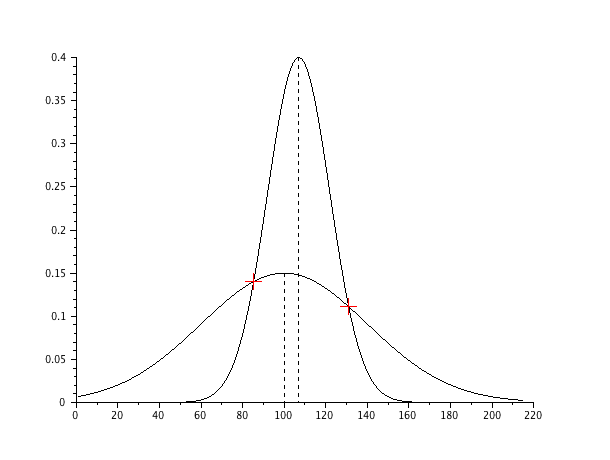
\includegraphics[width=.33\textwidth]{dessin_gauss/gmm_translation1.png}}
\subfloat[Cas limite, $\Delta c = C$]{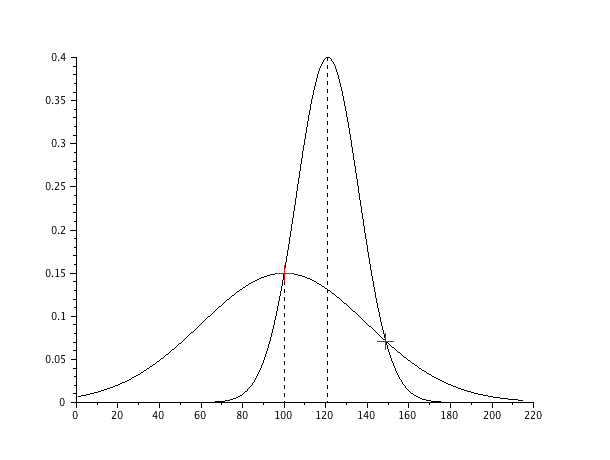
\includegraphics[width=.33\textwidth]{dessin_gauss/gmm_translation2.png}}
\subfloat[$\Delta c >C$]{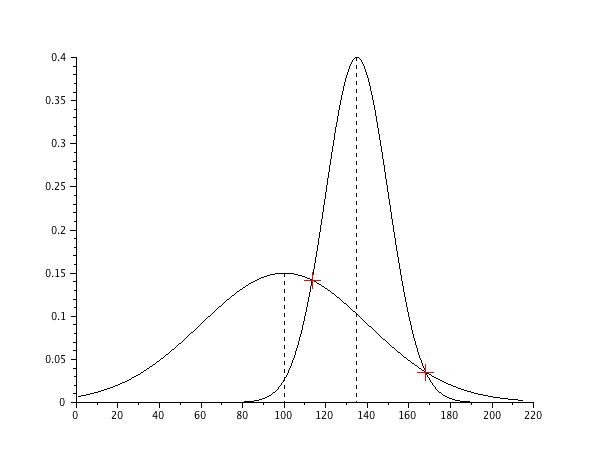
\includegraphics[width=.33\textwidth]{dessin_gauss/gmm_translation3.png}}
\caption{\label{fig:influence_dc} Influence de $\Delta c$ sur la position des points d'intersections (\mbox{$C=\max \left( -2\sigma_1^2 \ln(h_2/h_1) , 2\sigma_2^2 \ln(h_2/h_1) \right)$}).}
\end{figure}

\todo[inline]{Graphique ligne de niveaux, etc ...}

On peut voir l'influence de $\Delta c$ sur la position des points d'intersections.
\end{document}